\subsection{\cite{taubman2005musichand}}

In this paper, Taubman attempts to improve on notation input for professional musicians, allowing them to input rough ``sketched'' music and convert it into a neatly printed form. The application created, ``MusicHand'' makes use of a graphics tablet connected to a desktop machine and records the individual strokes the user makes.

Strokes are captured individually but using a latency threshold which is then used to group them together, adjusted on a per user basis. Taubman then makes use of statistical moments \todo{Reference to Moments Tech background} to classify these stroke groups, then making use of a K-NN algorithm to classify the object as one of several musical entities using the generated moments.

\begin{figure}[h]
  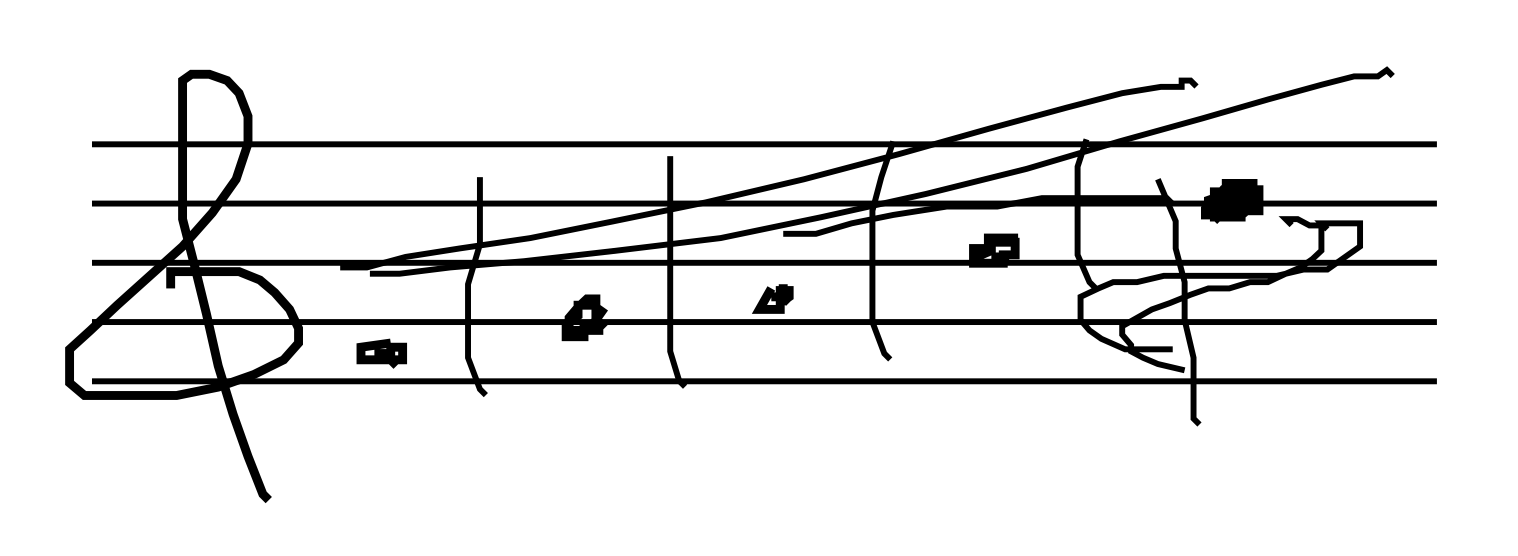
\includegraphics[width=\linewidth/2]{gfx/prior-research/taubman-sketch.png}
  \centering
  \caption{Example notation sketch from \cite{taubman2005musichand}}
  \label{fig:taubman-sketch}
\end{figure}

Since strokes are generally sketched as seen in \ref{fig:taubman-sketch} the application also makes use of a great deal of domain expertise, covered further in \todo{Domain Expertise Reference}, essentially running through a large flow chart in order to classify the entities further. However, the system notably relies on the compatibility of the generated moment ``libraries'' between users, a study of which was recommended for any future work but not done in this case. It is also suggested that instead of a graphics tablet, one might experiment with a more direct input method such as drawing onto a tablet directly with a stylus, the author specifically mentions the ``Wacom Cintiq''\footnote{http://uk.shop.wacom.eu/products/cintiq}, a ``digital canvas'' of sorts, which might allow a much more natural pen-paper feel.

